
\begin{frame}
    \frametitle{Geometric approach}
    \begin{columns}
        \begin{column}{0.5\textwidth}
            \begin{figure}
                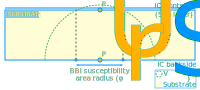
\includegraphics[width=\textwidth]{geomCrossViewNew.pdf}
            \end{figure}
        \end{column}
        \begin{column}{0.5\textwidth}
            \begin{figure}
                \includegraphics[width=\textwidth]{geomCrossViewThinNew.pdf}
            \end{figure}
        \end{column}
    \end{columns}
\end{frame}

\begin{frame}
    \frametitle{Geometric approach}
    \begin{columns}
        \begin{column}{0.5\textwidth}
            \begin{figure}
                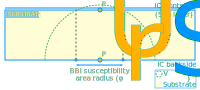
\includegraphics[width=\textwidth]{geomCrossViewNew.pdf}
            \end{figure}
        \end{column}
        \begin{column}{0.5\textwidth}
            \begin{figure}
                \includegraphics[width=\textwidth]{geomCrossViewThinNew2.pdf}
            \end{figure}
        \end{column}
    \end{columns}
\end{frame}

\begin{frame}{Geometric approach outcomes}
    \begin{enumerate}
        \setlength\itemsep{2em}
        \item Thinning the substrate → Reduce the voltage pulse for a given susceptibility area;
        \item Thinning the substrate → Susceptibility area increases at constant voltage;
        \item Thinning the substrate → No improvement in resolution.
    \end{enumerate}
\end{frame}
